\documentclass{article}
\usepackage[utf8]{inputenc}
\usepackage[english]{babel}
\usepackage{hyperref}

\usepackage{graphicx}
\usepackage{float}
\graphicspath{{figures/}}

\usepackage{todonotes}
\let\oldtodo\todo
\renewcommand{\todo}[1]{\oldtodo[noline]{#1}}

\usepackage{amsmath}
\usepackage{amssymb}
% \usepackage{amsthm}
\usepackage{commath}
\newcommand{\RR}{\mathbb{R}}
\newcommand{\NN}{\mathbb{N}}
\newcommand{\ZZ}{\mathbb{Z}}
\newcommand{\T}[1]{#1^{\top}}
\newcommand{\kth}[2][k]{#2^{(#1)}}
\DeclareMathOperator{\diag}{diag}
\DeclareMathOperator*{\argmin}{arg min}

\newcounter{summary}[section]
\newcommand{\summary}[1]{%
  \paragraph{\arabic{section}.\arabic{summary}\enspace #1.}\refstepcounter{summary}}
\renewcommand{\thesummary}{\thesection .\arabic{summary}}

\usepackage{tocloft}
\setcounter{tocdepth}{4}
\cftsetindents{paragraph}{0ex}{5ex}

\hyphenation{Lip-schitz}

\title{Summary of OCS Slides}
\author{Philipp Gabler}
\date{}

\begin{document}
\maketitle

\tableofcontents
\newpage

%%%%%%%%%%%%%%%%%%%%%%%%%%%%%%%%%%%%%%%%%%%%%%%%%%%%%%%%%%%%%%%%%%
\noindent First of all, the \href{http://web.mit.edu/6.252/www/LectureNotes/}{material} by the
course of Dimitri P. Bertsekas cover pretty much the same material. What a coincidence.

\section{Introduction}

\summary{General Form}

A general minimization problem has the form
\begin{equation*}
  \min_{x} f(x) \quad \text{s.t. } x \in X,
\end{equation*}
for a \emph{constraint set} \(X \subseteq \RR^n\) (often given by some \emph{constraint functions}
and an \emph{objective function} \(f: X \to \RR\).  We want to find an optimal value or
\emph{minimizer} \(x^* \in X\) such that
\begin{equation*}
  f(x^*) \leq f(x), \quad \forall x \in X.
\end{equation*}


\summary{Types of Optimization Problems}

\begin{enumerate}
\item
  \begin{enumerate}
  \item Discrete: \(X\) is a discrete set, also called \emph{interger programming}.
  \item Continuous: \(X\) is continuous (ie. uncountable)
  \end{enumerate}
\item
  \begin{enumerate}
  \item Linear: Objective functions and constraints are all linear:
    \begin{equation*}
      \min_x \T{c} x, \quad\text{s.t. } Ax \leq b,\; x \geq 0.
    \end{equation*}
    Constraints describe a polyhedron.  Efficiently solvable.
  \item Quadratic: Objective function is quadratic, constraints linear:
    \begin{equation*}
      \min_x \frac{1}{2}\T{x} Q x + \T{c} x, \quad\text{s.t. } Ax \leq b,\; Ex = d.
    \end{equation*}
    If \(Q\) is positive semidefinite, the objective is convex and the problem is polynomially
    solvable.
  \item Nonlinear: no further constraints.
  \end{enumerate}
\item
  \begin{enumerate}
  \item Unconstrained: Optimal solution searched in full \(\RR^n\). Easier to characterize, and
    usually to solve.
  \item Constrained: Optimal solution in an admissible region, usually more difficult to
    setup/characterize.
  \end{enumerate}
\end{enumerate}


\summary{Definiteness}

A symmetric matrix \(Q\) is called \emph{positive semidefinite} if \(\T{x} Q x \geq 0\) for all
\(x\), and \emph{positive definite} if \(\T{x} Q x > 0\) for all \(x \neq 0\).  Sometimes this is
written as \(Q \succeq 0\) and
\(Q \succ 0\).\footnote{\url{https://en.wikipedia.org/wiki/Positive-definite_matrix}} In the case of
\(Q \in \RR^{2 \times 2}\), we can use the following criteria:
\begin{enumerate}
\item \(Q \succeq 0 \Leftrightarrow \det Q \geq 0, Q_{11} \geq 0, Q_{22} \geq 0\) 
\item \(Q \succ 0 \Leftrightarrow \det Q > 0, Q_{11} > 0 \Leftrightarrow \) all eigenvalues of \(Q\)
  are positive.
\end{enumerate}


\summary{Convexity}

A set \(X\) is convex, if for all \(x, y \in X\) and \(\alpha \in [0,1]\):
\begin{equation*}
  \alpha x + (1 - \alpha) y \in X.
\end{equation*}
This means that \(X\) contains all convex combinations of points from it.


\summary{Convex Functions}

If \(X\) is a convex set, then \(f: X \to \RR\) is called convex if for all \(x, y \in X\) and
\(\alpha \in [0,1]\):
\begin{equation*}
  f(\alpha x + (1 - \alpha) y) \leq \alpha f(x) + (1 - \alpha) f(y).
\end{equation*}
This means that no points lie below any tangent.  Equivalent to this are the first-order condition
\begin{equation*}
  f(x) \geq f(y) + \T{\nabla f(y)}(x - y), \quad \forall x, y \in X
\end{equation*}
and the secon-order condition
\begin{equation*}
  \nabla^2 f(x) \succeq 0 \quad \forall x \in X.
\end{equation*}


\summary{Level Sets}

For an objective function \(f: X \to \RR\), and \(c \in \RR\), the sets
\begin{equation*}
  S_c(f) = \{x \in X: f(x) = c\}
\end{equation*}
are called \emph{level sets} of \(f\). They can be convex even if \(f\) is not!


\summary{Local and Global Minima}

A point \(x^*\) is called an \emph{unconstrained global minimum} of \(f\) if for all \(x\)
\begin{equation*}
  f(x^*) \leq f(x).
\end{equation*}
\(x^*\) is called an \emph{unconstrained local minimum} of \(f\) if it is minimal in some
neighbourhood; i.e., there is an \(\epsilon > 0\) such that
\begin{equation*}
  f(x^*) \leq f(x) \quad \forall x \text{ with } \lVert x^* - x \rVert \leq \epsilon.
\end{equation*}
For \emph{constrained} minima, we just require additionally that \(x \in X \subset \RR^n\).


\summary{First Order Neccessary Condition for Optimality}

In a small neighbourhood of \(x^*\), we can by Taylor expansion write \(f\) as
\begin{equation*}
  f(x) = f(x^* + \Delta x) = f(x^*) + \T{\nabla f(x^*)} \Delta x + o(\lVert \Delta x \rVert).
\end{equation*}
Since \(x^*\) is a local minimum, \(f(x^* + \Delta x) - f(x^*) \geq 0\), and we have
\begin{equation*}
  f(x^*) + \T{\nabla f(x^*)} \Delta x - f(x^*) = \T{\nabla f(x^*)} \Delta x \geq 0.
\end{equation*}
Since wlog. we can choose \(\Delta x\) to have the opposite sign, it holds also that
\begin{equation*}
  \T{\nabla f(x^*)} \Delta x \leq 0,
\end{equation*}
so \(\T{\nabla f(x^*)} \Delta x = 0\), which, since \(\Delta x\) is arbitrary, implies that
\(\nabla f(x^*) = 0\).


\summary{Second Order Neccessary Condition for Optimality}

By second order Taylor expansion, we get
\begin{align*}
  0 &\leq f(x^* + \Delta x) - f(x^*) \\
    &= f(x^*) + \underbrace{\T{\nabla f(x^*)} \Delta x}_{= 0} +
      \frac{1}{2} \T{\Delta x} \nabla^2 f(x^*) \Delta x + o(\lVert \Delta x \rVert^2) - f(x^*) \\
    &=  \frac{1}{2} \T{\Delta x} \nabla^2 f(x^*) \Delta x + o(\lVert \Delta x \rVert^2).
\end{align*}
From this follows that \(\T{\Delta x} \nabla^2 f(x^*) \Delta x \geq 0\).  Since \(\Delta x\) is
arbitrary, this means that \(\nabla^2 f(x^*)\) must be positive semidefinite.

A point which has this property is called a \emph{stationary point}.  In ``normal'' cases, it is
either a local optimum or a saddle point.


\summary{Sufficient Condition for Optimality}

If for a point \(x^*\) we have \(\T{\nabla f(x^*)} = 0\) and \(\nabla^2 f(x^*)\) positive
\emph{definite} (no ``semi-''!), then \(x^*\) is a strict unconstrained local minimum of f.


\summary{Minima of Convex Functions}

For a convex function \(f\), local minima are also global minima: suppose \(x*\) were a local, but
not global minimum. Then there must be some \(y^* \neq x^*\) with \(f(y^*) < f(x^*)\).  By
convexity, we have for all \(\alpha \in [0, 1)\):
\begin{equation*}
  f(\alpha x^* + (1 - \alpha) y^*) < \alpha f(x^*) + (1 - \alpha) f(y^*) < f(x^*),
\end{equation*}
which contradicts the assumption, so \(x^*\) must also be a global minimum.

Furthermore, the neccessary condition for minima, \(\nabla f(x^*) = 0\), for convex functions
becomes a sufficient condition.\todo{why this?}


%%%%%%%%%%%%%%%%%%%%%%%%%%%%%%%%%%%%%%%%%%%%%%%%%%%%%%%%%%%%%%%%%%
\section{Gradient Methods}

\summary{Basic Idea}\label{s:gradient_methods}

To find a minimum of \(f\), we construct a sequence \(\kth{x}\) such that for all \(k\),
\(f(\kth[k+1]{x}) < f(\kth{x})\).  To do that, we choose an initial \(\kth[0]{x}\) and then set
\begin{equation*}
  \kth[k+1]{x} = \kth{x} + \kth{\alpha} \kth{d}.
\end{equation*}
Here \(\kth{\alpha}\) is some step size, and \(\kth{d}\) is a \emph{descent direction} which must
satisfy
\begin{equation*}
  \pd{f}{{\kth{d}}}(\kth{x}) = \T{\nabla f(\kth{x})} \kth{d} < 0, 
\end{equation*}
where \(\pd{f}{{\kth{d}}}\) is the directional derivative in direction \(\kth{d}\).


\summary{Matrix-Scaled Gradients}

Given the above form, one can choose \(\kth{d} = -\kth{D} \nabla f(\kth{x})\) for a positive
definite \(\kth{D}\):
\begin{equation*}
  \T{\nabla f(\kth{x})} \kth{d} = -\T{\nabla f(\kth{x})} \kth{D} \nabla f(\kth{x}) < 0,
\end{equation*}
by the definition of positive definiteness.

\begin{enumerate}
\item Steepest descent: \(\kth{D} = I\). Simple, but slow convergence.
\item Newton's method: \(\kth{D} = (\nabla^2 f(\kth{x}))^{-1}\).  Fast convergence, but
\(\nabla^2 f(\kth{x})\) needs to be positive definite to be invertible.  Corresponds to local
approximation by a quadratic surface (see below). \todo{references to later sections}
\item Levenberg-Marquart method: \(\kth{D} = (\nabla^2 f(\kth{x}) + \lambda I)^{-1}\).  Tries
to fix problems with Newton's method by regularization.
\item Diagonal scaling: \(\kth{D} = \diag(\kth{d}_1, \ldots, \kth{d}_n)\). E.g. approximating
Newton's method with
\begin{equation*}
  \kth{d}_i = \left( \pd[2]{f}{x_i}(\kth{x}) \right)^{-1}.
\end{equation*}
\item Gauss-Newton method: For a nonlinear least-squares problem
\(f(x) = \frac{1}{2} \lVert g(x) \rVert^2\), we can choose
\(\kth{D} = ( \nabla g(\kth{x} \T{\nabla g(\kth{x})})^{-1}\).  This is related to the
pseudo-inverse.
\end{enumerate}


\summary{Step Size Selection}

To ensure convergence and performance, \(\kth{\alpha}\) needs to be chosen with care.
Theoretically, it is not enough set it such that \(f(\kth[k+1]{x}) < f(\kth{x})\); there are
counterexamples for which this holds, but \(\lim_{, \to \infty} f(\kth{x}) > f(x^*)\), e.g., when
the step sequence in the limit oscillates between two values on the opposite sides of a ``bowl''.

Some usual approaches to choosing the step size are:
\begin{enumerate}
\item Minimization rule: choose \(\kth{\alpha}\) such that the minimum in the descent direction is
  taken, i.e.
  \begin{equation*}
    f(\kth{x} + \kth{\alpha}\kth{d}) = \min_{\alpha \geq 0} f(\kth{x} + \alpha\kth{d}).
  \end{equation*}
\item Limited minimization rule: ``heuristically'' search the best \(\kth{\alpha}\) in some set,
  like in an interval \([0, s]\) or among some values \(\{\beta^0 s, \beta^1 s, \ldots \}\) for some
  fixed \(\beta \in (0, 1)\) and \(s > 0\).
\item Constant step size: sometimes, an optimal (or good enough) value \(\kth{\alpha} = s\) can be
  computed from the objective function in advance.
\item Diminishing step size: choose a decreasing sequence with
  \(\lim_{k \to \infty} \kth{\alpha} = 0\) and \(\sum_{k = 0}^{\infty} \kth{\alpha} = \infty\).  The
  latter is sufficient to ensure convergence (we can never ``run out of space'' before the optimum
  is reached).  This has good theoretical properties for some setups, but the convergence rate can
  be quite slow.
\end{enumerate}


\summary{Armijo Rule}

This is a special method for step size selection, which has nice theoretical properties (e.g. using
it, the \(\kth{x}\) always converge to a stationary point).  To apply it, we fix scalars \(s\), \(0 <
\beta < 1\), and \(0 < \sigma < 1\), and set \(\kth{\alpha} = \beta^{m_k} s\), where we choose
\(m_k\) as the first nonnegative integer for which
\begin{equation*}
  f(\kth{x} + \beta^{m_k} s \kth{d}) - f(\kth{x}) \leq \sigma \beta^{m_k} s \nabla \T{f(\kth{x})} \kth{d}.
\end{equation*}

The interpretation of this is that we try out the step sizes \(\beta^{m_k} s\) in decreasing order,
until we find one for which the decrease in the objective is sufficiently large (see
Fig.~\ref{fig:armijo}).

\begin{figure}[h]
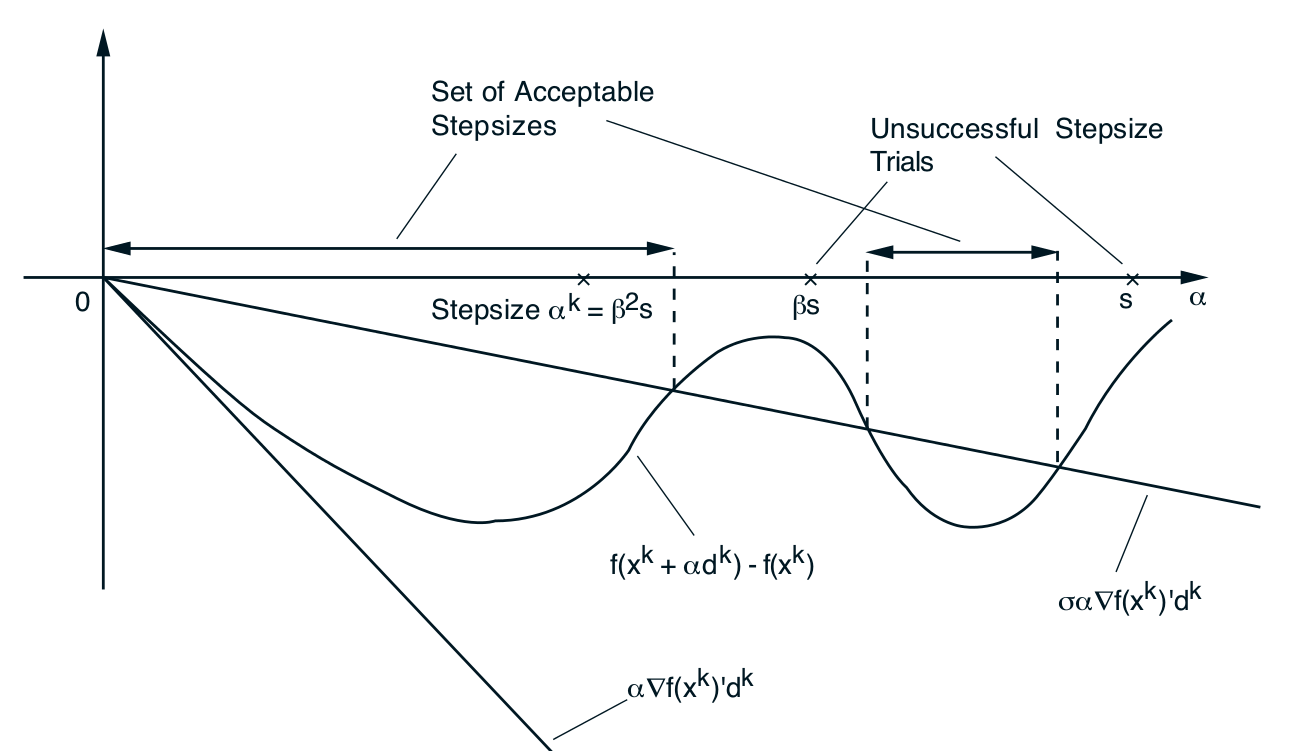
\includegraphics[width=\textwidth]{armijo.png}
\caption{Graphical interpretation of Armijo rule.\label{fig:armijo}}
\end{figure}


\summary{Termination of Gradient Methods}

Gradient methods are not automatically convergent, so we need some stopping criterion.  The standard
approach is to terminate iteration based on the norm of the gradient:
\begin{equation*}
  \lVert \nabla f(\kth{x}) \rVert \leq \epsilon,
\end{equation*}
for some reasonable \(\epsilon > 0\).  Since the absolute sizes of the gradients are not
neccessarily meaningful, a better criterion is
\begin{equation*}
  \frac{\lVert \nabla f(\kth{x}) \rVert}{\lVert \nabla f(\kth[0]{x}) \rVert} \leq \epsilon.
\end{equation*}
Assuming we have diagonal scaling, we can also use
\(\lVert \kth{D} \nabla f(\kth[0]{x}) \rVert \leq \epsilon\).

If \(\nabla^2 f(x)\) is positive definite, we have a strongly convex problem, and the norm of the
gradient actually bounds the distance to a local minimum \(\enVert{x - x^*}\).


%%%%%%%%%%%%%%%%%%%%%%%%%%%%%%%%%%%%%%%%%%%%%%%%%%%%%%%%%%%%%%%%%%
\section{Convergence Analysis}

\summary{Gradient Related Condition}

A sequence of descent directions \(\{\kth{d}\}\) is called \emph{gradient related} to a step
sequence \(\{\kth{x}\}\), if for any subsequence \(\{\kth{x}\}_{k \in \mathcal{K}}\) converging to a
nonstationary point, the corresponding subsequence \(\{\kth{d}\}_{k \in \mathcal{K}}\) is bounded
and satisfies
\begin{equation*}
  \limsup_{k \in \mathcal{K} \to \infty} \T{\nabla f(\kth{x})} \kth{d} < 0.
\end{equation*}
The interpretation of this is that in the limit, \(\kth{d}\) is still a descent direction (see
Summary~\ref{s:gradient_methods}).

This is, for example, satisfied for \(\kth{d} = -\kth{D}\nabla f(\kth{x})\), when the eigenvalues of
\(\kth{D}\) are bounded between zero and a positive constant.  It fails if the directions get more
and more orthogonal to the gradient; a counterexample would be a sequence which oscillates in the
limit, due to a badly chosen step size (there, all finite directions are descent directions, but
they get ``worse'' in the limit).


\summary{Lipschitz continuity}

A continuously differentiable function \(f: \RR^n \to \RR\) is called \emph{Lipschitz continuous},
if there is value \(L \geq 0\), called \emph{Lipschitz constant}, such that for all \(x, y \in
\RR^n\) and \(t \in [0, 1]\):
\begin{equation*}
  \enVert{\nabla f(x + ty) - \nabla f(x)} \leq Lt \enVert{y}.
\end{equation*}
Intuitively, a Lipschitz continuous function is limited in how fast it can change: there exists a
Lipschitz constant such that, for every pair of points on the graph of this function, the absolute
value of the slope of the line connecting them is not greater than this
constant.\footnote{\url{https://en.wikipedia.org/wiki/Lipschitz_continuity}}

A function \(\RR \to \RR\) is Lipschitz continuous with \(L = \sup_x |g'(x)|\) if and only if it has
bounded first derivative.


\summary{Descent Lemma}\label{s:descent_lemma}

Let \(f: \RR^n \to \RR\) be Lipschitz continuous with Lipschitz constant \(L\).  Then for all
\(x, y\), we have the following quadratic upper bound on the objective function at \(x\):
\begin{equation*}
  f(x + y) \leq f(x) + \T{\nabla f(x)}y + \frac{L}{2}\enVert{y}^2.
\end{equation*}

Derivation: let \(g(t) = f(x + ty)\) for \(t \in [0, 1]\).
\begin{align*}
  f(x + y) - f(x) &= g(1) - g(0) \\
                  &= \int_0^1 \dod{g}{t}(t) \dif t \\
                  &= \int_0^1 \T{\nabla f(x + ty)} y \dif t \\
                  &= \int_0^1 \T{\nabla f(x)} y \dif t
                    + \int_0^1 \left( \T{\nabla f(x + ty)} - \T{\nabla f(x)} \right) \cdot y \dif t \\
                  &\overset{(1)}{\leq} \int_0^1 \T{\nabla f(x)} y \dif t
                    + \int_0^1 \enVert[1]{\nabla f(x + ty) - \nabla f(x)}\! \cdot \enVert[1]{y} \dif t \\
                  &\overset{(2)}{\leq} \T{\nabla f(x)} y + \enVert[1]{y} \int_0^1 Lt\enVert[1]{y} \dif t \\
                  &= \T{\nabla f(x)} y + \frac{L}{2}\enVert[1]{y}^2,
\end{align*}
where (1) is an application of the Cauchy-Schwarz theorem
(\(\langle x, y \rangle \leq \enVert{x} \cdot \enVert{y}\)), and (2) follows from Lipschitz
continuity.


\summary{Interpretation of Descent Lemma}\label{s:descent_lemma_interpretation}

We can express the lemma in terms of a step sequence \(\{\kth{x}\}\) by substituting
\(\{x \mapsto \kth{x}, y \mapsto (x - \kth{x})\}\):
\begin{equation*}
  f(x) \leq f(\kth{x}) + \T{\nabla f(\kth{x})}(x - \kth{x}) + \frac{L}{2}\enVert[1]{x - \kth{x}}^2.
\end{equation*}
This is actually a local upper bound of \(f\) at \(x\) by a quadratic function, which we can
optimize analytically by derivation:
\begin{gather*}
  \nabla f(\kth{x}) + L (x - \kth{x}) \overset{!}{=} 0\\
  \quad \Rightarrow x = \kth{x} - \frac{1}{L} \nabla f(\kth{x})
\end{gather*}
Convergent step size methods relate to this fact.


\summary{Convergence with Constant Step Size}

Assume \(f\) is Lipschitz continuous, and \(\{\kth{x}\}\) is a sequence generated by a gradient
method with gradient related \(\kth{d} \neq 0\).  The we have
\begin{align*}
  f(\kth{x} + \kth{\alpha}\kth{d}) - f(\kth{x})
  &\leq \overbrace{\T{\nabla f(\kth{x})} \kth{d}}^{< 0} \kth{\alpha} +
    \frac{1}{2} (\kth{\alpha})^2 L \enVert[1]{\kth{d}}^2 \\
  &= \underbrace{\kth{\alpha} \left( \frac{1}{2} \kth{\alpha} L \enVert[1]{\kth{d}}^2
    - \envert[1]{\nabla f(\kth{x}) \kth{d}} \right)}_{A}.
\end{align*}
We first calculate the optimal step size \(\kth{\bar{\alpha}} = \min_{\kth{\alpha}} A\):
\begin{gather*}
  \dpd{A}{{\kth{\alpha}}} = (\kth{\alpha})^2 L \enVert[1]{\kth{d}}^2 - \envert[1]{\T{\nabla
                            f(\kth{x})} \kth{d}} \overset{!}{=} 0 \\
  \Rightarrow \kth{\bar{\alpha}} = \enVert[1]{\kth{d}} - \frac{\envert[1]{\T{\nabla
                       f(\kth{x})} \kth{d}}}{(\kth{\alpha})^2 L \enVert[1]{\kth{d}}^2}
\end{gather*}
Then, for general \(\kth{\alpha}\) with
\(\epsilon \leq \kth{\alpha} \leq (2 - \epsilon)\kth{\bar{\alpha}}\), we have
\begin{align*}
  f(\kth{x} + \kth{\alpha}\kth{d}) - f(\kth{x})
  &\leq \kth{\alpha} \left( \frac{1}{2} L \enVert[1]{\kth{d}}^2
    - \envert[1]{\T{\nabla f(\kth{x})} \kth{d}} \right) \\
  &\leq \kth{\alpha} \left( \frac{1}{2} (2 - \epsilon)\; \frac{\envert[1]{\T{\nabla
    f(\kth{x})} \kth{d}}}{(\kth{\alpha})^2 L \enVert[1]{\kth{d}}^2} L \enVert[1]{\kth{d}}^2
    - \envert[1]{\T{\nabla f(\kth{x})} \kth{d}} \right) \\
  &= \kth{\alpha} \left( \envert[1]{\T{\nabla f(\kth{x})} \kth{d}}
    - \frac{\epsilon}{2} \envert[1]{\T{\nabla f(\kth{x})} \kth{d}}
    - \envert[1]{\T{\nabla f(\kth{x})} \kth{d}} \right) \\
  &= \kth{\alpha} \underbrace{\left( -\frac{\epsilon}{2}\envert[1]{\T{\nabla f(\kth{x})} \kth{d}}
    \right)}_{\leq 0};
\end{align*}
and by the reverse,
\begin{align*}
  f(\kth{x} + \kth{\alpha}\kth{d}) - f(\kth{x})
  &\geq \kth{\alpha} \left(\frac{\epsilon}{2}\envert[1]{\T{\nabla f(\kth{x})} \kth{d}} \right) \\
  &\geq \frac{\epsilon^2}{2}\envert[1]{\T{\nabla f(\kth{x})} \kth{d}},
\end{align*}
where the last step results from the assumption about \(\kth{\alpha}\).  Thus,
\(f(\kth{x}) \geq f(\kth[k+1]{x}) \geq \cdots \); in each step, the function is decreased by at
least \(\frac{\epsilon^2}{2}\envert[1]{\T{\nabla f(\kth{x})} \kth{d}}\).

Convergence to a stationary point follows by contradiction: assume a subsequence
\(\{\kth{x}\}_{k \in \mathcal{K}}\) converged to a point \(\bar{x}\) which is non-stationary (ie.,
for which \(\nabla f(\bar{x}) \neq 0\)).  From above, we know that
\begin{equation*}
  f(\kth{x} + \kth{\alpha}\kth{d}) - f(\kth{x}) \to 0
\end{equation*}
(assuming \(f\) is bounded below), and by that
\begin{equation*}
\envert[1]{\T{\nabla f(\kth{x})} \kth{d}} \to 0  
\end{equation*}
This would however contradict to \(\kth{d}\) being gradient related, since it implies
\begin{equation*}
  \limsup_{k \in \mathcal{K} \to \infty} \T{\nabla f(\kth{x})} \kth{d} = 0
\end{equation*}
Therefore, every accumulation point \(\bar{x}\) of \(\{\kth{x}\}\) must be stationary
(\(\nabla f(\bar{x}) = 0\)).


\summary{Convergence with Armijo Rule}
\todo{TODO}


\summary{Convergence Rates}

Important for practical problems, to compare different algorithms.  Is usually measured in terms of
a step-dependent error function \(e: \RR^n \to \RR\) with \(e(x^*) = 0\).  Common choices are
\begin{equation*}
  e(x) = \enVert[1]{x - x^*}, \quad\text{or} \\
  e(x) = f(x) - f(x^*)
\end{equation*}
We are interested in the asymptotic behaviour of \(e\), in terms of how much better the method
improves for every step.  We have:
\begin{enumerate}
\item Sublinear convergence, if for all \(k\)
  \begin{equation*}
    \limsup_{k \to \infty} \frac{e(\kth[k+1]{x})}{e(\kth{x})} = 1.
  \end{equation*}
\item Linear convergence, if for all \(k\)
  \begin{equation*}
    \limsup_{k \to \infty}
    \frac{e(\kth[k+1]{x})}{e(\kth{x})} \leq \beta \in (0, 1).
  \end{equation*}
\item Superlinear convergence, if for all \(k\)
  \begin{equation*}
    \limsup_{k \to \infty} \frac{e(\kth[k+1]{x})}{e(\kth{x})} = 0.
  \end{equation*}
  (which does not imply that the method does not converge!)
\end{enumerate}
Alternatively, we can compare \(e\) to a standard sequence of powers: if there exist \(q > 0\),
\(\beta \in (0, 1)\), and \(p \geq 1\) such that
\begin{equation*}
  e(\kth{x}) \leq q \beta^{p^k},
\end{equation*}
we have linear convergence if \(p = 1\), and superlinear convergence of order \(p\) if \(p > 1\).
The latter is equivalent to
\begin{equation*}
  \limsup_{k \to \infty} \frac{e(\kth[k+1]{x})}{e(\kth{x})^p} < \infty.
\end{equation*}
\todo{derivations for some rates? analysis of quadratic model?}


%%%%%%%%%%%%%%%%%%%%%%%%%%%%%%%%%%%%%%%%%%%%%%%%%%%%%%%%%%%%%%%%%%
\section{Newton's Method and Variants}

\summary{Basic Idea}

A second order method, which is one of the fastest gradient methods.  We generate the sequence
\(\{\kth{x}\}\) based on
\begin{equation*}
  \kth[k+1]{x} = \kth{x} - \kth{\alpha}\left( \nabla^2 f(\kth{x}) \right)^{-1} \nabla f(\kth{x}),
\end{equation*}
where we assume that the direction \((\nabla^2 f(\kth{x}))^{-1} \nabla f(\kth{x}\) is
defined and a descent direction.

This has three problems when we are far from a local minimum:
\begin{enumerate}
\item The Hessian can be singular~-- we what are reasonable approximations in this case?
\item The Hessian is convex~-- it attracts local maxima as well as minima.  Thus, we must choose the
  step size carfully.
\item The direction might not be a descent direction.
\end{enumerate}
Variants of the method deal with this, to ensure convergence globally while maintaining the fast
convergence rate.


\summary{Derivation of Newton's Method from Taylor Expansion}

By Taylor approximation: Given a point \(\kth{x}\), we can approximate a function
\(f \in \mathcal{C}^2\) locally as
\begin{equation*}
  f^k(x) = f(\kth{x}) + \T{\nabla f(\kth{x})}(x - \kth{x})
  + \frac{1}{2} \T{(x - \kth{x})} \nabla^2 f(\kth{x})(x - \kth{x}).
\end{equation*}
Compare this to the Descent Lemma (Summary~\ref{s:descent_lemma_interpretation})~-- there,
\(\nabla^2 f\) is approximated by \(L\), with some transformation of the metric.

We can analytically minimize this approximation, which gives the stated update rule:
\begin{align*}
  \nabla f^k(x) = \nabla f(\kth{x}) + \nabla^2 f(\kth{x})(x - \kth{x}) &\overset{!}{=} 0 \\
  \nabla^2 f(\kth{x})(x - \kth{x}) &= -\nabla f(\kth{x}) \\
  (x - \kth{x}) &= -(\nabla^2 f(\kth{x}))^{-1} \nabla f(\kth{x}) \\
  x = \kth[k+1]{x} &= \kth{x} - (\nabla^2 f(\kth{x}))^{-1} \nabla f(\kth{x}).
\end{align*}


\summary{Relation of Newton's Method to Equation Solving}

The general for of Newton's method is not used for optimization, but for solving equations of the
form \(g(x) = 0\), where \(g: \RR^n \to \RR^n \in \mathcal{C}^1\).  For this problem, the method has
the form
\begin{equation*}
  \kth[k+1]{x} = \kth{x} - (\T{\nabla g(\kth{x})})^{-1} g(\kth{x}).
\end{equation*}
A method converging to a stationary point results from setting \(g(x) = \nabla f(x)\), implying a
symmetric matrix \(\T{\nabla g(x)} = \nabla^2 f(x)\).


\summary{Local convergence}

For a local optimum \(x^*\) of \(f\), we must have \(\nabla f(x^*) = 0\), or, by the above relation
to equation solving, \(g(x^*) = 0\).  Now, suppose \(\kth{x} \to x\) and \(\nabla f(x^*)\) is
nonsingular.  Expanding \(g\) around \(x^*\), we get
\begin{equation*}
  0 = g(x^*) = g(\kth{x}) + \T{\nabla g(\kth{x})} (x^* - \kth{x}) + o\!\del[1]{\,\enVert[1]{x^* - \kth{x}}};
\end{equation*}
multiplying from the left with \((\T{\nabla g(\kth{x})})^{-1}\), this is
\begin{gather*}
  \kth{x} - x^* - (\T{\nabla g(\kth{x})})^{-1} g(\kth{x}) = \kth[k+1]{x} - x^* = o\!\del[1]{\,\enVert[1]{x^* - \kth{x}}} \\
  \Rightarrow \quad \lim_{k \to \infty} \frac{\enVert[1]{\kth[k+1]{x} - x^*}}{\enVert[1]{\kth{x} - x^*}} = 0,
\end{gather*}
therefore we have superlinear convergence.


\summary{Global Convergence by Diagonal Modifications}

To solve the problems mentioned above, when we are far away from an optimum, we can add a diagonal
matrix \(\kth{\Delta}\) to the Hessian, such that \(\nabla^2 f(\kth{x}) + \kth{\Delta} \succ 0\).
In that way, we the Newton equation
\begin{equation*}
  \left( \nabla^2 f(\kth{x}) + \kth{\Delta} \right) \kth{d} = -\nabla f(\kth{x})
\end{equation*}
can be solved, and \(\kth{d}\) is a descent direction.  Some possibilities for \(\kth{\Delta}\) are
simply a large enough multiple of \(I\), or more advanced methods like modified Cholesky
factorization\footnote{\url{https://www.gnu.org/software/gsl/manual/html_node/Modified-Cholesky-Decomposition.html}}
or a combination of a dampening factor with a trust
region\footnote{\url{https://en.wikipedia.org/wiki/Trust_region}}.


%%%%%%%%%%%%%%%%%%%%%%%%%%%%%%%%%%%%%%%%%%%%%%%%%%%%%%%%%%%%%%%%%%
\section{Least Squares Optimization and Model Fitting}

\summary{General Form}

We want to minimize a function
\begin{equation*}
  f(x) = \frac{1}{2} \enVert[1]{g(x)}^2 = \frac{1}{2} \sum_i \enVert[1]{g_i(x)}^2,
\end{equation*}
for a continuously differentiable function \(g\) with components \(g_i\), which can be linear or
nonlinear.  This is equivalent to solving the problem \(g(x) = 0\).


\summary{Gauss-Newton Method}

To get a step method, we replace \(g(x)\) by a local approximation around \(\kth{x}\):
\begin{equation*}
  \tilde{g}(x, \kth{x}) = g(\kth{x}) + \T{\nabla g(\kth{x})}(x - \kth{x}).
\end{equation*}
Then we have a quadratic problem:
\begin{align*}
  \kth[k+1]{x} &= \argmin_{x \in \RR^n} \frac{1}{2} \enVert[1]{\tilde{g}(x, \kth{x})}^2 \\
               &= \argmin_{x \in \RR^n} \frac{1}{2} \enVert[1]{g(\kth{x}) + \T{\nabla g(\kth{x})}(x -
                 \kth{x})}^2 \\
  \Rightarrow\hspace{1.125cm} 0 &\overset{!}{=} \frac{1}{2} \left( \enVert[1]{g(\kth{x})}^2
      + 2\T{(x - \kth{x})} \nabla g(\kth{x}) g(\kth{x})
      + \T{(x - \kth{x})} \nabla g(\kth{x}) \T{\nabla g(\kth{x})} g(\kth{x}) \right) \\
  \Rightarrow\quad \kth[k+1]{x} &= \kth{x} - \left(\nabla g(\kth{x}) \T{\nabla
                                  g(\kth{x})}\right)^{-1}
                                  \nabla g(\kth{x}) g(\kth{x}),
\end{align*}
assuming that \((\nabla g(\kth{x}) \T{\nabla g(\kth{x})}\) is invertible.


\summary{Levenberg-Marquardt Method}

To ensure that \((\nabla g(\kth{x}) \T{\nabla g(\kth{x})}\) is invertible, and the descent direction
is actually gradient related, one can use a modified iteration
\begin{equation*}
  \kth[k+1]{x} = \kth{x} - \kth{\alpha}\left(\nabla g(\kth{x}) \T{\nabla g(\kth{x})} + \kth{\delta} I\right)^{-1}
  \nabla g(\kth{x}) g(\kth{x}),
\end{equation*}
where \(\kth{\alpha}\) can be chosen by the Armijo rule, and \(\kth{\delta} > 0\).


\summary{Connection of Gauss-Newton to Newton}

The target function of a least squares problem, \(f(x) = \frac{1}{2}\enVert[0]{g(x)}^2\), with
components \(g_i\), has derivatives
\begin{align*}
  \nabla f(x) &= \T{\nabla g(x)} g(x), \\
  \nabla^2 f(x) &= \nabla g(x) \T{\nabla g(x)} + \sum_i \nabla^2 g_i(x) g_i(x).
\end{align*}
Neglecting the second-order part in the Hessian, this reduces to a form equivalent to Newton's
method, but saving the computation of the Hessian (intuitively, \(\nabla^2 g \approx (\nabla g)^2\)).


\summary{Incremental Gradient Methods}

Usually, a least squares problem is a model fitting problem, where \(g_i(x) = z_i - h(y_i, x)\), for
a model function \(h\) with parameters \(x\), samples \(y_i\), and targets and \(z_i\).  Thus, we
can see each \(g_i\) as a data block, and \(g = (g_1, \ldots, g_m)\) as the data set.  (In machine
learning terminology, this corresponds to stochastic gradient descent with minibatches for ``data
blocks''.)

If the data set is large, the Gauss-Newton iterations are costly (because the matrix to be inverted
becomes large).  Sometimes, for example in real-time applications, the data samples also are not
provided in advance, but only incrementally.  Therefore, we can use the following scheme to
calculate updates based on single samples:
\begin{align*}
  \kth{\xi}_0 &= \kth{x} \\
  \kth{\xi}_i &= \kth{\xi}_{i-1} - \kth{\alpha} \nabla g_i(\kth{\xi}_{i-1}) g_i(\kth{\xi}_{i-1}) \\
  \kth[k+1]{x} &= \kth{\xi}_m.
\end{align*}
This amounts to
\begin{equation*}
  \kth[k+1]{x} = \kth{x} - \kth{\alpha} \sum_i \nabla g_i(\kth{\xi}_{i-1}) g_i(\kth{\xi}_{i-1}),
\end{equation*}
where we base the update on the intermediate \(\kth{\xi}_i\) instead of using the full gradient
\begin{equation*}
  \nabla f(\kth{x}) = \sum_i \nabla g_i(\kth{x}) g_i(\kth{x}).
\end{equation*}
This converges very fast in the first iterations, but needs further restictions on the step size to
ensure global convergence.


\summary{Kalman Filter}

If the model (ie. the functions \(g_i\)) is linear, one Gauss-Newton iteration is enough to find the
least squares estimate (this amounts to the analytical solution using the Moore-Penrose
pseudoinverse).  However, we can develop an incremental method for this, avoiding the matrix
inversion.  This method is called \emph{Kalman filter}.

Suppose \(g_i(x) = z_i - C_i x_i\), with \(z_i \in \RR^r\) and \(C_i \in \RR^{r \times n}\) (the
model parameters).  We are interested in a method for finding
\begin{equation*}
  \xi_i \in \argmin_x \sum_{j=1}^{i} \lambda^{i-j} \enVert[1]{z_j - C_j x}.
\end{equation*}
The optimal solution is then \(x^* = \xi_m\).  For \(\lambda = 1\), this is the least squares fit;
for \(\lambda < 1\), we ``decay'' the importance of ``older'' samples.  The sequence of \(\xi_i\)
can be generated iteratively by
\begin{align*}
  \xi_i &= \xi_{i-1} + H_i^{-1}\T{C_i}(z_i - C_i \xi_{i-1}), \quad\text{with} \\
  H_i &= \lambda H_{i-1} + \T{C_i}C_i, \\
  H_0 &= 0,\quad \xi_0 \text{ arbitrary}.
\end{align*}
(\(H_i\) and \(C_i\) are relatively small, compared to \(\nabla f(\kth{x})\).)

Example: for a linear model \(x(t) = l + ft\), with parameters \(f, l\), we use \(C = [1, t]\).


\summary{Extended Kalman Filter}

If the \(g_i\) are nonlinear, we can use a linearization at the last available iteration
\(\xi_{i-1}\) to get the \emph{extended Kalman filter}:
\begin{gather*}
  \tilde{g}_i(x, \xi_{i-1}) = g_i(\xi_{i-1}) + \T{\nabla g_i(\xi_{i-1})}(x - \xi_{i-1}), \\
  \xi_i \in \argmin_x \sum_{j=1}^{i} \lambda^{i-j} \enVert[1]{\tilde{g}_j(x, \xi_{i_1})}.
\end{gather*}
The iteration scheme stays the same, but we have to adapt the model parts to
\begin{align*}
  \tilde{z}_i &= \tilde{g}_i(z_i, \xi_{i-1}), \\
  C_i &= - \T{\nabla g_i(\xi_{i-1})}.
\end{align*}


%%%%%%%%%%%%%%%%%%%%%%%%%%%%%%%%%%%%%%%%%%%%%%%%%%%%%%%%%%%%%%%%%%
\section{Accelerated Gradient Methods}

\summary{Lower Bound for Quadratic Optimization}


\end{document}
